%%%%%%%%%%%%%%%%%%%%% chapter.tex %%%%%%%%%%%%%%%%%%%%%%%%%%%%%%%%%
%
% sample chapter
%
% Use this file as a template for your own input.
%
%%%%%%%%%%%%%%%%%%%%%%%% Springer-Verlag %%%%%%%%%%%%%%%%%%%%%%%%%%

\chapter{Sistemi Adattivi}
Fin ora per la classificazione abbiamo utilizzato strumenti che derivano dall'analisi statistica, adesso invece il problema verrà affrontato dal punto di vista di emulazione del comportamento celebrale. Conosciamo ben poco di come può essere il comportamento celebrale umano, studi in neuropsicologia e neuropsichiatria hanno condotto ad un analisi abbastanza ampia dei comportamenti celebrali in virtù di stimoli che ispirano ad una serie di modelli. Il modello che descriveremo non è ispirato a statistica e probabilità, ma sono soltanto ispirazioni all'analisi emotiva. Ciò porta a progettare un sistema adattativo, che può essere visto come una scatola nera in quanto non si conosce il comportamento interno ma si conosce l'output di un determinato input. Il sistema è detto adattivo in quanto il sistema riesce ad apprendere per esperienza, è in grado di modificare se stesso in funzione delle coppie input-output desiderato. Tutto ciò è possibile grazie ad un \emph{tuning} cioè alla modifica dei parametri del sistema adattativo. Questo aggiornamento dei parametri verrà sempre indicato con una freccia obliqua come mostrato in figura \ref{sa}.
\begin{figure}
\centering
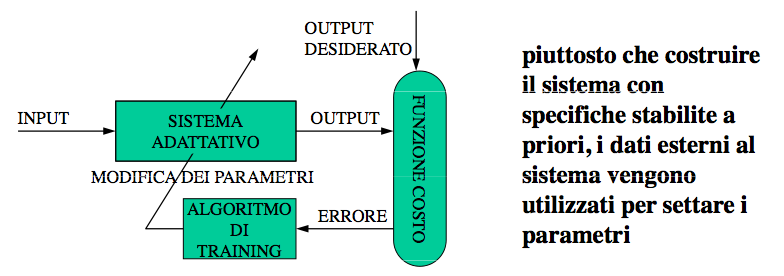
\includegraphics[scale=0.5]{img/sistema_adattativo.png}
\caption{Sistema adattativo}
\label{sa}
\end{figure}
In breve, una volta fornito l'input ed ottenuto l'output si va a misurare quanto si scosta dall'output desiderato e per modificare i parametri ci si basa sull'errore commesso.  Da ora in poi la modifica dei parametri verrà chiamata in modo arbitrario come \emph{learning} dei parametri o \emph{training} dei parametri. Per misurare l'errore dobbiamo disporre di una funzione costo che deve essere minimizzata, o in alternativa massimizziamo la risposta (quanto l'utente è soddisfatto del risultato prodotto rispetto a quello che si attendeva?). \'E la funzione costo che guida l'apprendimento. Nel caso supervised conosciamo l'input ed il corrispondente output, conosciamo la funzione costo, conosciamo il sistema adattativo, l'unica cosa che non è nota sono i parametri che vanno appresi. L'obiettivo è quello di progettare un sistema che sia in grado di modificare i parametri in modo tale che dato un input produca un output molto vicino a quello desiderato. Se a questo sistema aggiungiamo anche la conoscenza della struttura interna del sistema stesso allora stiamo parlando di un sistema adattivo secondo il principio neurale. Oltre all'apprendimento dei parametri viene appresa anche la struttura del sistema.  I modelli che andremo a studiare sono modelli di tipo formale, quindi cerchiamo di formalizzare un modello che deriva da un sistema fisico reale (fig. \ref{modello}). 
\begin{figure}
\centering
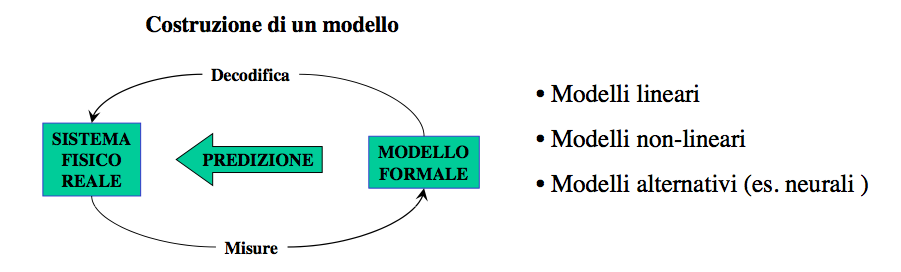
\includegraphics[scale=0.5]{img/modello.png}
\caption{Costruzione di un modello}
\label{modello}
\end{figure}
Ci sono due modi di operare, il primo è quello di partire dal sistema fisico reale, e prendere delle misure per modellare il modello formale, l'altro invece è quello di partire dal modello formale e ritornare a decodificare il sistema fisico reale. Tanto per fare un esempio uno dei modelli lineari più noti è quello che cerca di fare il fitting dei dati utilizzando la regressione lineare. La regressione lineare è quella che praticamente cerca di stimare la funzione che soggiace i punti (fig. \ref{regressione}),
\begin{figure}
\centering
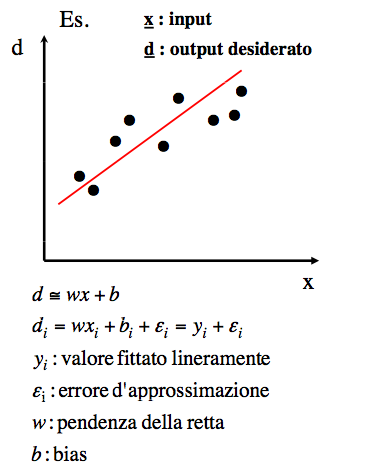
\includegraphics[scale=0.6]{img/regressione.png}
\caption{Regressione lineare}
\label{regressione}
\end{figure}
Effettuare un fitting troppo eccessivo porta ad un sistema che ha poca capacità di generalizzazione. L'ideale sarebbe quello di trovare una funzione per la quale gli stessi punti sono rumore, l'errore medio esiste sempre ma essendo distribuito su tutti i punti sarebbe minore, quindi capacità di generalizzazione. Questa tecnica ispirò ad uno dei primi modelli adattativi, l' adaline (fig. \ref{adaline}).
\begin{figure}
\centering
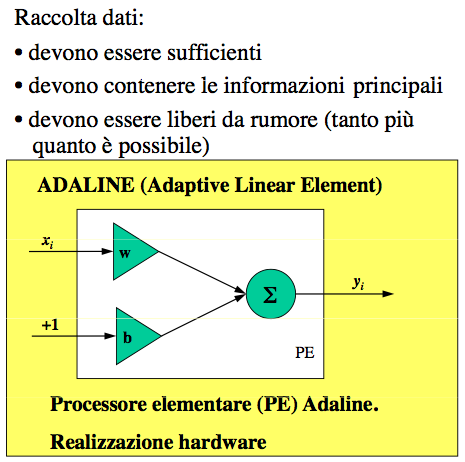
\includegraphics[scale=0.5]{img/adaline.png}
\caption{Adaline}
\label{adaline}
\end{figure}
L'adaline opera proprio come una regressione lineare, l'obiettivo è quello di trovare la funzione lineare parametrizzata. La progettazione dell'adaline è composta da tre elementi: due moltiplicatori $\mathbf{w}$ e $\mathbf{b}$, il secondo prende il nome di \emph{bias}, viene poi considerata una sommatoria di prodotti (funzione lineare)
\begin{equation}
y_i =  \mathbf{w}_1\mathbf{x}_1 + \mathbf{w}_2 \mathbf{x}_2 + \dots + \mathbf{w}_n \mathbf{x}_n + \mathbf{b} 
\end{equation}
quindi
\begin{equation}
y_i = \sum_{i=1}^n \mathbf{w}_i \mathbf{x}_i + \mathbf{b}
\end{equation}
Il bias è quel valore che ci consente di inclinare l'iperpiano nello spazio mutidimensionale. La progettazione del sistema è nota, quello che non è noto è il valore di $\mathbf{w}$ e di $\mathbf{b}$. L'obiettivo è quello di individuare i parametri tali che ad un $\mathbf{x}_i$ in input venga fornito un $y_i$ in uscita. Se consideriamo $d \simeq wx + b$ il valore di output desiderato allora dobbiamo trovare $y_i$ che più si avvicina a $d$. 
\begin{equation}
d_i = wx_i + b_i + \varepsilon_i = y_i + \varepsilon_i
\end{equation}
quindi per far tendere $y$ a $d$ bisogna minimizzare $\varepsilon$, che è esattamente la differenza
\begin{equation}
\varepsilon_i = d_i - y_i = d_i - (wx_i + b)
\end{equation}
Questo è un classico problema che viene risolto con i minimi quadrati, quindi si va a minimizzare la somma dei quadrati degli scostamenti. Possiamo usare la funzione costo MSE (errore quadratico medio) normalizzato su tutti gli $n$ campioni. Indichiamo con $J$ la funzione costo
\begin{equation}
J = \frac{1}{2N} \sum_{i=1}^N \varepsilon_i^2
\end{equation}
dove $N$ è il numero di osservazioni. Sostituendo $\varepsilon_i$ si ottiene
\begin{equation}
J = \frac{1}{2N} \sum_{i=1}^N (d_i - (wx_i + b))^2
\end{equation}
Questa è una funzione costo parametrizzata, bisogna trovare $w$ tale che $J$ sia minimo. Per risolvere questo problema si usa la tecnica del gradiente discendente, quindi andiamo ad effettuare le derivate parziali di $J$ rispetto a $w$ e rispetto a $b$, le poniamo uguali a zero e risolviamo,  ottenendo 
\begin{gather}
b= \frac{\sum_i x_i^2 \sum_i d_i - \sum_i x_i \sum_i x_i d_i}{N \left[ \sum_i (x - \bar{x})^2 \right]}\\
w = \frac{\sum_i (x_i - \bar{x}) - (d_i - \bar{d})}{\sum_i (x_i - \bar{x})^2}
\end{gather}
e vediamo che dipendono da $\bar{x}$ e $\bar{d}$, quindi dal valor medio degli ingressi e dal valor medio delle uscite. Per poter fare apprendimento è necessario processare tutto il training set, uno svantaggio in termini di complessità. Riassumendo, ogni volta che viene fornita una coppia di input-output si misura l'errore, questi errori poi vengono accumulati e poi vengono utilizzati per determinare il valore di $w$ e di $b$. Un modo per misurare le prestazioni è quello di considerare il coefficiente di correlazione $r$, che non è altro che il rapporto tra la covarianza di due variabili casuali e il prodotto della due varianze(Fig \ref{coeff}). 
\begin{figure}[h]
\centering
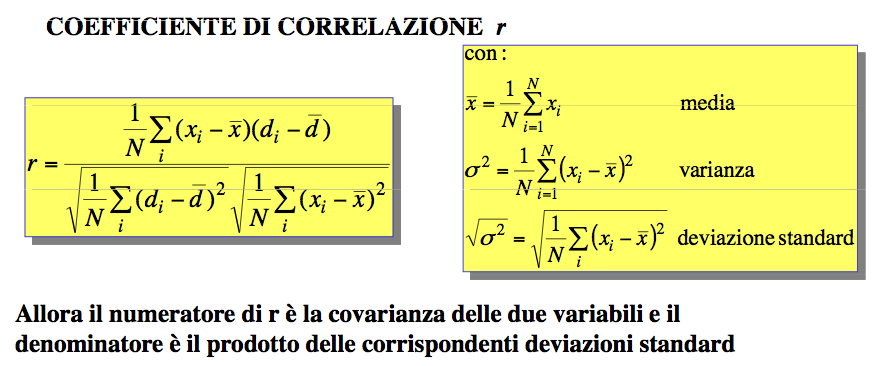
\includegraphics[scale=0.5]{img/coeff.png}
\caption{Coefficiente di correlazione}
\label{coeff}
\end{figure}
Possiamo misurare le performance del sistema osservando il coefficiente di correlazione che può assumere valori tra $-1$ e $1$. Un coefficiente pari a uno significa che c'è una correlazione perfetta tra quello che ci attendiamo e quello che viene prodotto ($x$ e $d$ covariano), quando il coefficiente vale $-1$ c'è una correlazione perfetta lineare negativa, quando il coefficiente è uguale a zero allora $x$ e $d$ sono scorrelate.

\section{Metodo del gradiente discendente}
\noindent Il gradiente discendente ha una particolarità,  se minimizzo il funzionale, supponendo che il funzionale abbia l'andamento rappresentato in figura \ref{gradiente}
\begin{figure}
\centering
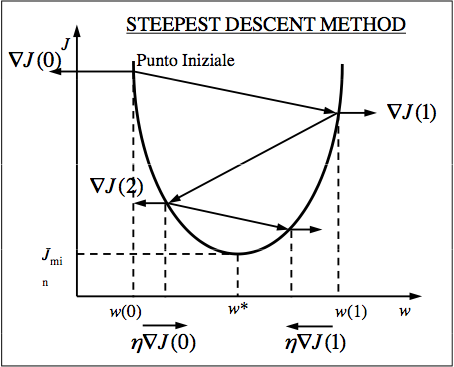
\includegraphics[scale=0.5]{img/gradiente.png}
\caption{Gradiente discendente}
\label{gradiente}
\end{figure}
tendiamo a raggiungere il punto minimo del funzionale $J_{min}$ rispetto al quale determiniamo il parametro.  Nel caso banale di un funzionale che dipende da un unico parametro che è $w$,  sull'asse delle ascisse vogliamo trovare quel valore di $w$ tale che si ottiene il valore della funzione costo minimo. L'idea è quella di partire da un punto qualsiasi ed arrivare a $w$ finale pattern dopo pattern, cioè dopo aver fornito un esperienza dopo esperienza, è un metodo di addestramento che è chiamato per epoche (insieme dei pattern). Quindi fornito un input, si vede il sistema come opera, si misura lo scostamento, si aggiorna il valore di $w$, e si fornisce un altra coppia di input output desiderato e si ripetere il procedimento finché non raggiungiamo il valore minimo di $J$. Ci accorgiamo di aver raggiunto il minimo quando il valore successivo del $J$ è maggiore di quello precedente, allora ci conserviamo il valore precedente di $J$ e quindi anche il parametro che ci ha condotto al valore minimo $w^*$. Il metodo del gradiente discendente è un metodo che viene applicato passo dopo passo, il metodo iterativo dice che il $w$ al passo uno è uguale al $w$ al passo 0 più l'incremento. Il gradiente non è altro che la normale, la tangente del punto della curva in cui lo sto calcolando, quindi fondamentalmente il gradiente è un vettore che ha una direzione che va in modo opposto alla curva, quindi se voglio andare nella direzione del minimo della funzione costo dobbiamo andare nella direzione opposta del gradiente. Per incrementare $w$ bisogna utilizzare la derivata parziale di $J$ rispetto a $w$,  ma l' incremento che è direttamente proporzionale al gradiente deve essere necessariamente nella direzione allora l'incremento diventa $-\nabla J$. Quindi
\begin{equation}
w(1) = w(0) - \eta \nabla J(0)
\end{equation}
dove $\eta$ è il tasso di apprendimento, che nel caso sia uguale ad uno allora tutto l'incremento viene utilizzato per l'aggiornamento, ma potrebbe causare che si arrivi al minimo $J$ in modo veloce. Il problema è che potrebbero esserci più minimi locali, ma a noi interessa ottenere il minimo globale, incrementando molto il valore di $w$ si potrebbe arrivare velocemente ad un minimo che potrebbe essere quello locale, il problema si risolve non incrementando tutto il valore di $w$. La regola generale 
\begin{equation}
w(k+1) = w(k) - \eta \nabla J(k)
\end{equation}
è chiamata la regola di adeline. Questa è una delle regole di aggiornamento più famose, da ora in poi verrà applicata in molti modi, questa formula è alla base dell'apprendimento. 

\section{Metodo Least Mean Square(LMS)}
Vediamo come viene applicato al metodo LMS, in precedenza abbiamo visto che la funzione costo è 
\begin{equation}
J = \frac{1}{2N} \sum_{i=1}^N \varepsilon_i^2 = \frac{1}{2N} \sum_{i=1}^N (d_i - wx_i)^2
\end{equation}
Calcoliamo poi la derivata parziale di $J$ rispetto a $w$ al passo $k$  ( la derivata di una sommatoria non è altro che la sommatoria delle derivate ) ed otteniamo
\begin{equation}
\nabla J(k) = - \varepsilon (k) \cdot x(k)
\end{equation}
Sostituendo nella regola generale di aggiornamento, otteniamo 
\begin{equation}
w(k+1) = w(k)- \eta \nabla J (k)_{stimato} = w(k) + \eta \varepsilon(k)x(k)
\end{equation}
quindi l'incremento del peso è direttamente proporzionale al prodotto dell'errore commesso e del pattern in ingresso. Questo tipo di apprendimento fatto passo dopo paso è detto apprendimento on-line. Se invece viene effettuato dopo aver misurato gli errori si tutti i pattern viene detto training batch. $\eta$ essendo un parametro può essere appreso anche lui durante la fase di apprendimento dei parametri ma con il rischio che i due apprendimenti possono sovrapporsi e far si che il sistema non vada a convergenza.

\section{Estensione a variabili multiple}
\'E la semplice estensione al caso d-dimensionale quindi la formula precedente viene riscritta in questo modo
\begin{equation}
y= \sum_{k=1}^d w_k x_k + b
\end{equation}
in questo caso non abbiamo più una retta di regressione lineare ma abbiamo un iperpiano. Il ragionamento è identico, non ho l'apprendimento di un solo peso, ma ho l'apprendimento di tanti pesi quante sono le variabili. In figura \ref{ndim} è rappresentato un esempio.
\begin{figure}
\centering
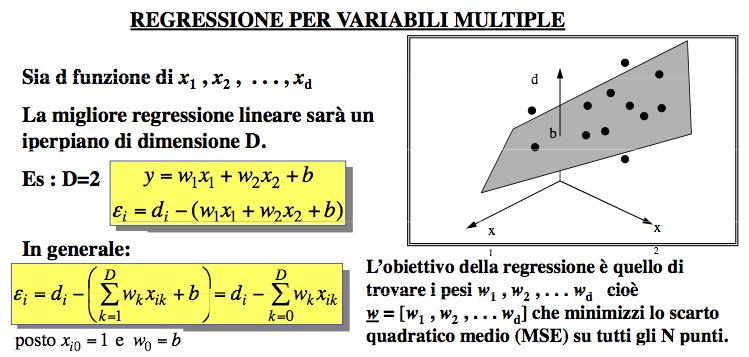
\includegraphics[scale=0.6]{img/caso_ndim.png}
\caption{Estensione a variabili multiple}
\label{ndim}
\end{figure}

\section{Processore Elementare PE (Adaline)}
Un adaline può anche essere un elemento di un sistema che è costituito da altri elementi principali, ed è detto processore elementare(PE). Mettendo insieme tanti adaline ho un sistema di PE. Nel calcolo parallelo può essere paragonato ad un sistema di tipo SIMD, quindi fanno tutti la stessa cosa ma su dati diversi. 
\begin{figure}
\centering
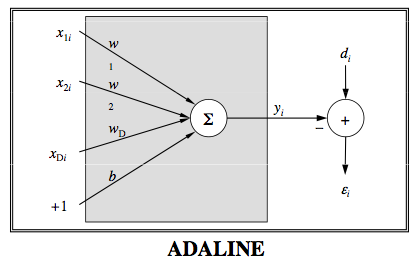
\includegraphics[scale=0.7]{img/adaline2.png}
\caption{Adaline}
\label{adaline2}
\end{figure}



%
